% DIFFERENT TYPES OF LISTS, FIGURES, AND REFERENCING (SECTIONS, FIGURES, ETC.)

\documentclass[14pt, a4paper]{article} %14 pt indicates the font size of the prepared document
\usepackage[utf8]{inputenc} %indicates the encoding of the document
\usepackage{color} %this package enables the use of colors.
\usepackage{graphicx}
\usepackage{subcaption}

\title{Template - Add Figure(s)}
\author{Kawshik Kumar Paul}
\date{\today}

\begin{document}
\maketitle
\tableofcontents %this command creates the table of contents with all numbered sections, subsections, etc.
\pagebreak %This will force the rest of the document to start in another page.

\section{Section 1}
\label{sec:intro} %This will be used while referencing this section
This is the introduction section.

This is an itemized list.
\begin{itemize}
    \item item 1
    \begin{itemize}
        \item nested item 1
        \item nested item 2
    \end{itemize}
    \item item 2
    \item item 3
\end{itemize}

\subsection{Subsection 1.1}
\label{subsec:1.1} %This will be used while referencing this subsection
This is subsection 1.1.

This is an enumerated list.
\begin{enumerate}
    \item First item
    \item Second item
    \item This can also be nested.
    \begin{enumerate}
        \item nested item 1
        \item nested item 2
    \end{enumerate}
\end{enumerate}

\subsubsection{Subsubsection 1.1.1}
This is subsubsection 1.1.1.

This is a descriptive list.
\begin{description}
\item[Number 1] one
\item[Number 2] two
\end{description}

\pagebreak 

\subsection*{Unnumbered subsection}
This is an unnumbered subsection under Introduction. 
\begin{figure}[h]
	\centering
	\caption{This caption is at the top}
	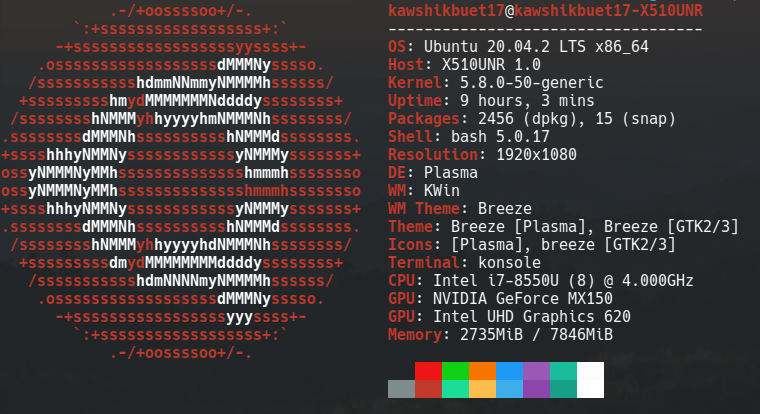
\includegraphics[scale=0.15]{figure1.jpg}
	\label{fig:1}
	\caption{This is figure 1.}
\end{figure}


\section*{Unnumbered Section Example}
This section should not be numbered. Using * after the section specifier prevents this numbering. This will NOT show up in the Table of Contents. 

Referencing the figure used above: \ref{fig:1}.

\pagebreak
\section{Page top figure}
\begin{itemize}
 \item Figure is on top
 \item This section is in same page of that Figure
\end{itemize}

\begin{figure}[t]
    \centering
    \caption{This is top caption}
    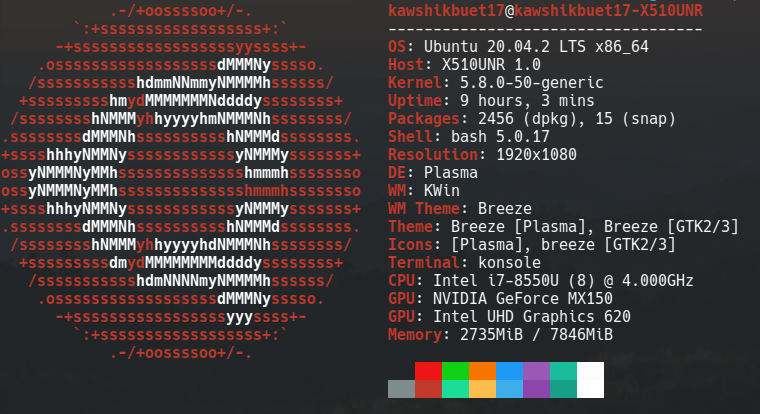
\includegraphics[scale=0.2]{figure1.jpg}
    \caption{This is bottom caption}
\end{figure}


\pagebreak
\section{Page bottom figure}
\begin{itemize}
 \item Figure is on bottom
 \item This section is in same page of that Figure
 \item b is botton and b! is bottom override
\end{itemize}

\begin{figure}[b!]
    \centering
    \caption{This is top caption}
    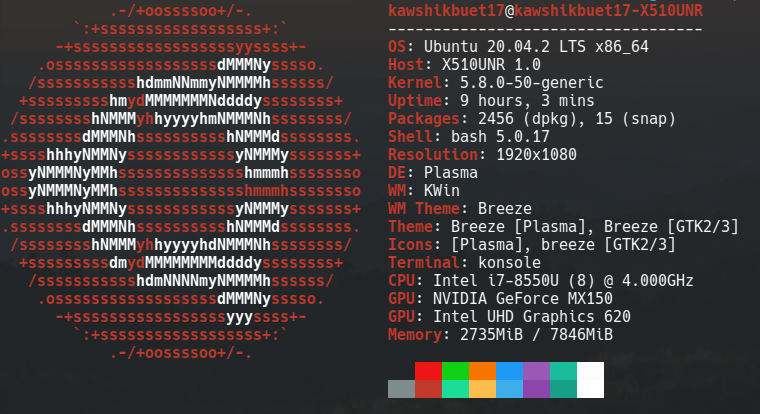
\includegraphics[scale=0.4]{figure1.jpg}
    \caption{This is bottom caption}
\end{figure}


\pagebreak
\section{Multiple Figure}
    \subsection{Multiple Figure 1}
        \begin{figure}[h!]
            \centering
            \begin{subfigure}[b]{0.4\linewidth}
                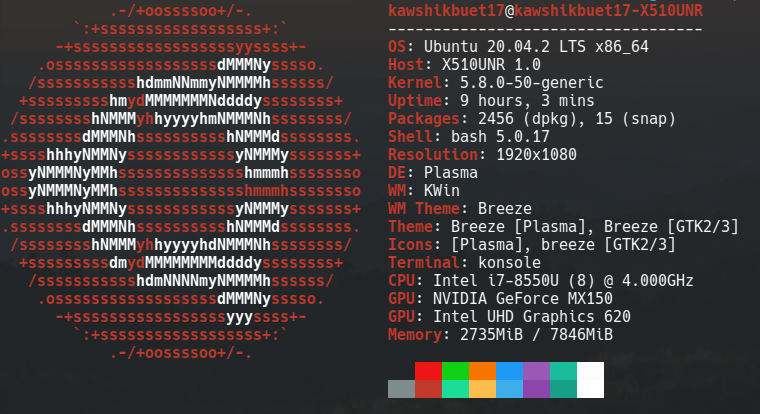
\includegraphics[width=\linewidth]{figure1.jpg}
                \caption{fig.}
            \end{subfigure}
            \begin{subfigure}[b]{0.4\linewidth}
                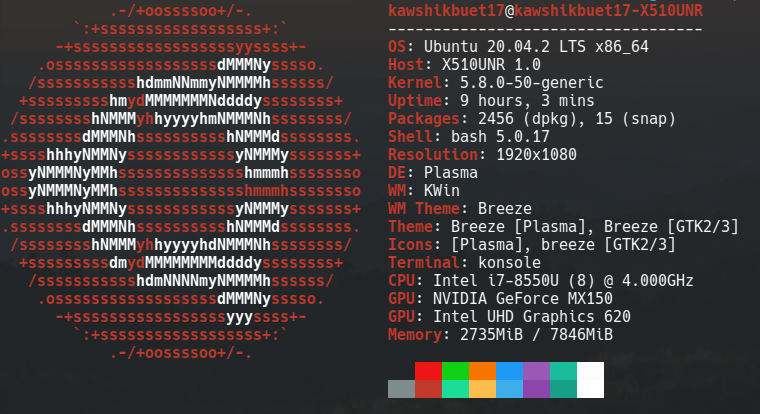
\includegraphics[width=\linewidth]{figure1.jpg}
                \caption{More fig.}
            \end{subfigure}
            \caption{The same figure. Two times.}
        \end{figure}
        
    \subsection{Multiple Figure 2}
        \begin{figure}[h!]
            \centering
            \begin{subfigure}[b]{0.2\linewidth}
                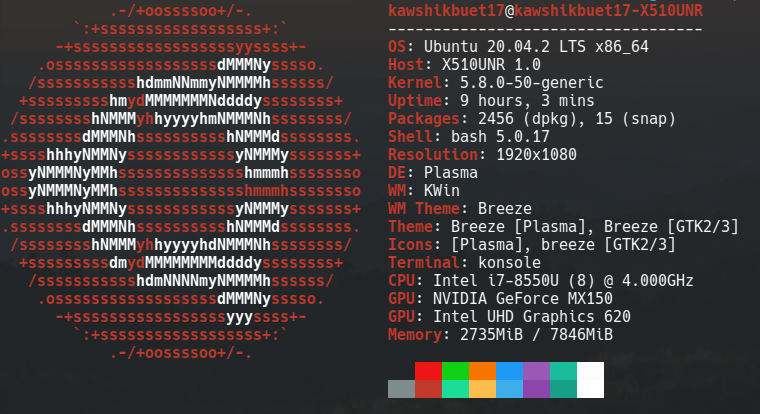
\includegraphics[width=\linewidth]{figure1.jpg}
                \caption{fig.}
            \end{subfigure}
            \begin{subfigure}[b]{0.2\linewidth}
                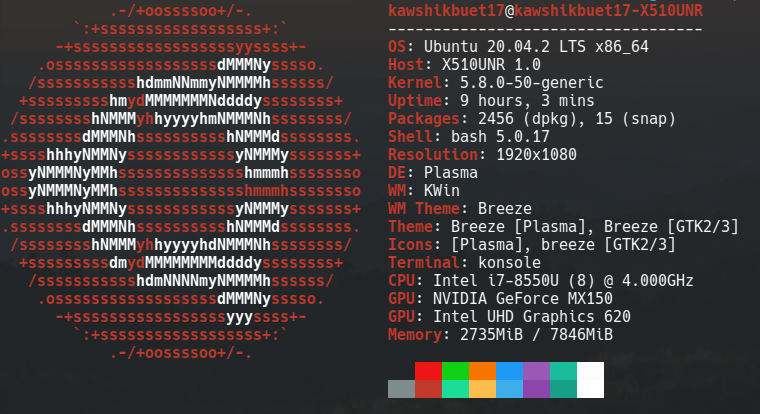
\includegraphics[width=\linewidth]{figure1.jpg}
                \caption{More fig.}
            \end{subfigure}
            \begin{subfigure}[b]{0.2\linewidth}
                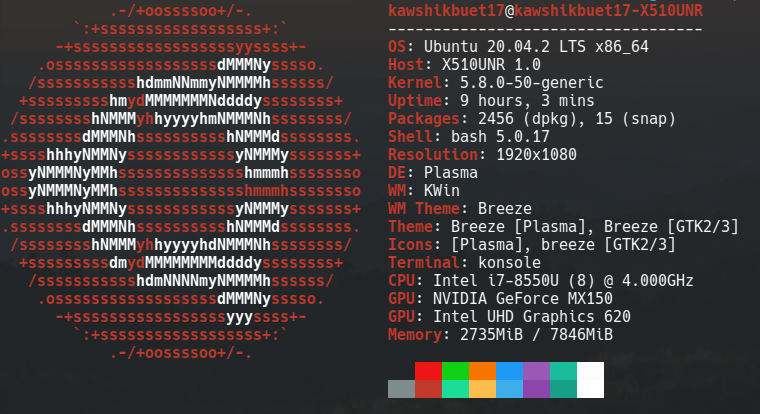
\includegraphics[width=\linewidth]{figure1.jpg}
                \caption{More fig.}
            \end{subfigure}
            \begin{subfigure}[b]{0.5\linewidth}
                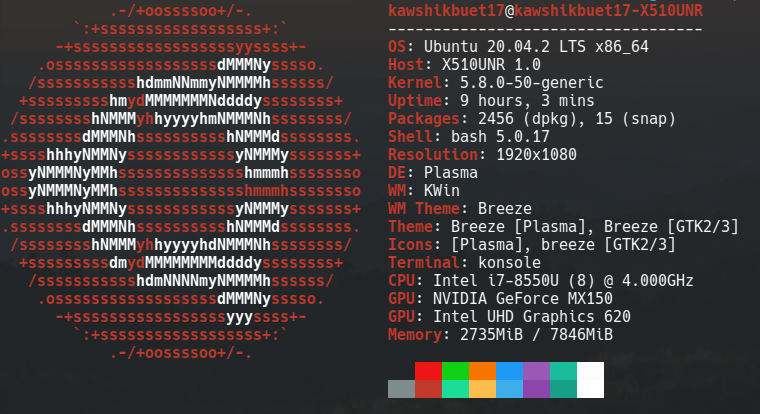
\includegraphics[width=\linewidth]{figure1.jpg}
                \caption{Too much fig.}
            \end{subfigure}
            \caption{The same figure. Multiple times.}
            \label{fig:coffee3}
        \end{figure}
\end{document}
